\subsection{Geometry editor}
\writer{Mikko}

The Geometry editor is the component used to define lines and points in two dimensional plane which will then define the shape of the visualized simulation. Figure \ref{fig:model-geometry} describes the geometry model used by the Geometry Editor.

\begin{figure}[htp]
\begin{center}
  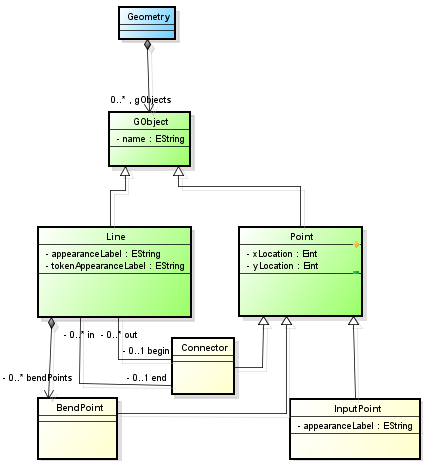
\includegraphics[width=0.8\textwidth]{image/geometry_diagram.png}
  \caption{Geometry domain model}
  \label{fig:model-geometry}
\end{center}
\end{figure}

\paragraph{Geometry}
The Geometry class is an abstract definition of a geometry object.

\paragraph{GObject}
The GObject is a geometry object, which can be either a line or a point. It has attribute \textbf{name}. It is used to name individual geometry objects, so that user can easily tell them apart. Furthermore, it is used as identifier for all geometry objects.

\paragraph{Point}
Point is a location in the two dimensional plane. It has attributes \textbf{xLocation} and \textbf{yLocation} which refer to the horizontal and vertical coordinates respectively.

\paragraph{InputPoint}
Class InputPoint refers to objects that will be clickable for the user in the 3D simulation. \textbf{AppearanceLabel} is used to identify the 3d appearance of InputPoint, such as traffic light, tree, planet etc, within simulation.

\paragraph{Connector}
Class Connector is either the beginning or the ending parametric point of a line. Therefore, lines that end at a Connector are \textbf{in} and lines that start from a Connector are \textbf{out}.

\paragraph{BendPoint}
Class BendPoint is the type of parametric point that define the curvature of the line.

\paragraph{Line}
Class Line is a parametric curve in a two dimensional plane. The line begins at a point location \textbf{begin} and it ends at a point location \textbf{end}. A \textbf{BendPoint} is a point location which parametrically defines the curvature of the line, unless it doesn't have one, thus the line would be straight. \textbf{AppearanceLabel} Is used to define the 3d shape of the line within 3d simulator. The appearance will be extrapolated along the length of the line, thus the appearance could for instance be track, road, empty space, etc.
